\documentclass[12pt,a4paper]{journal}
\usepackage[margin=1in]{geometry}

\usepackage[utf8]{inputenc}
\usepackage[T1]{fontenc}
\usepackage{indentfirst}
\usepackage{amsmath}
\usepackage{amsfonts}
\usepackage{amssymb}
\usepackage{caption}
\usepackage{subcaption}
\usepackage{graphicx}
\usepackage{siunitx}
\sisetup{range-phrase=--, range-units=single}

\graphicspath{{img/}}
\usepackage[numbers, square]{natbib}


\begin{document}

\section{Retinal haemodynamics, vascular disease, neovascular AMD and diabetic retinopathy}

\subsection{Retinal haemodynamics}

In the retina, two separate circulatory systems, namely the inner retinal vasculature and the choroid, are charged with bringing oxygen to the cells.
The inner retinal vasculature is composed of one to four separate vascular complexes, depending on the location, and is absent in a \SI{0.5}{\mm} wide circular region at the centre of the retina called the fovea.
The choroid is composed of three vascular layers.
The caliber of the vessels in each layer decreases as it gets closer to the retina.
The inner most layer is called the choriocapillaris and is made of capillaries aranged within a single plane, parallel to the retinal plane.
While the inner retinal vasculature is embedded inside the retinal tissue, the choroid lies behind the retina, to which it is linked through Bruch's membrane.
Bruch's membrane is a thin (\SIrange{2}{4}{\micro\meter}) structure mediating exchanges of gases and biological by-products between the retina and the choroidal circulation.
The retinal vasculature typically feeds the inner \SIrange{60}{80}{\percent} of the retina, while the choroid supplies the remaining, more metabolically active, outer layers around the photoreceptors~\cite{Birol_2007}.

Retinal haemodynamic models are concerned with simulating blood flow within the choroid and the inner vasculature of the retina.
Adequate blood flow is essential to ensure delivery of nutrients and oxygen to the retinal cells.
Haemodynamic models are concerned with describing the properties of blood within a vascular network.
In the case of the retina, this vascular network can be either the inner retinal vasculature or the choroid.
Blood flow across a vessel is determined by the difference in blood pressure on each end of the vessel, its length, the size of the cross section of its lumen, the region between the vessel walls where blood flows.
These properties of a vessel define the vascular resistance that is opposing the flow of blood.
In addition, external pressures exert forces against the vessel walls, increasing vascular resistance.

Constant blood flow can be maintened by the vessels by varying the vascular resistance in response to changes in the environment, e.g., changes in incoming flow during physical exercise or external pressures.
This ability of the vasculature is called autoregulation.
Both the retinal and choroidal circulation are able to autoregulate blood flow.
In the inner retinal vasculature, arteries close to the central retinal artery are surrounded by 5 to 7 layers of smooth muscle cells.
Those cells can act on an artery's radius to increase vascular resistance and maintain constant blood flow.
The number of smooth muscle cells decreases as the arterioles branch into capillaries and venules, with only a sparse number of those cells on venules larger than \SI{10}{\micro\meter}~\cite{An2020, Kur_2012}.
% As the arteries branch, the amount of smooth muscle cells diminishes.
% In arterioles of diameter \SIrange{8}{15}{\micro\meter}, only a single layer of smooth muscle cells is found while the walls of capillaries and venules are devoid of such cells. 
% Only a sparse number of smooth muscle cells is found on the walls of veins of diameter larger than \SI{10}{\micro\meter}.
This organisation suggests that blood flow in the retina is regulated mainly by arteries and arterioles.
Evidence suggests that the choroid is also able, maybe to a lesser degree, to autoregulate blood flow~\cite{CERiva1997, Polska2007}.

A number of mechanisms act on the tone of smooth muscle cells lining the vessel walls, effectively contracting or dilatating the vessel.
For a review of those mechanisms observed \textit{in vivo}, see~\cite{Kur_2012}.
In a number of retinal diseases such as neovascular age-related macular degeneration (nAMD) and diabetic retinopathy (DR), ocular blood flow and blood flow regulation have been observed to be impaired, see~\cite{Kur_2012} and references therein.

While direct \textit{in vivo} measurements of blood flow are possible, they are difficult to achieve and accurate data remains limited, especially in the choroid.
In addition, current imaging and measurement modalities do not provide insights on the regulation pathways leading to changes in ocular blood flow.
Mathematical models of the haemodynamics of ocular blood flow can help understand the relationships between IOP, systemic blood pressure, blood gases and oxygen availability in the retina.
Some of the properties of blood flow seen in Equation~\ref{eq:PoiseuilleLaw} and the stress generated on the vessel walls are difficult to measure \textit{in vivo}.
Vessel radius and length can be estimated straightforwardly from images of the retina~\cite{DoblhoffDier2014}.\\
Fundus photography is one of those imaging modalities, displaying the whole retina but with limited resolution of smaller vessels.
Injection of dye prior to the photography is possible to better highlights blood vessels and leakage of blood.\\
Optical coherence tomography (OCT) is another modality.
During OCT scans, a light beam with long wavelength is sent to the retina and resulting backscattered light is compared to a control beam.
Comparison of the signals provides a three-dimensional view of the retinal tissue.
The scans can be used to infer the presence of blood flow, that is blood vessels, and is termed OCT angiography (OCTA).
The OCTA technique uses a decorelation algorithm on two OCT scans to highlight movement of particles.
In the case of the retina, the only movement comes from red blood cells in suspension in the bloodstream.
OCTA provides high resolution scans of the vasculature within the desired field of view, which is not limited to the whole retina.
However, leakages are not shown on OCTA as they are static structures.\\
The choroid lies behind the retina and therefore, is hidden on photographs of the retina.
While OCTA is able to image the choroid, accuracy is limited by artefacts caused by the presence of blood vessels in the retina.
Therefore, \textit{in vivo} quantification of the choroidal circulation is more complicated than the retinal circulation.

\textit{In silico}, blood can be modeled as an incompressible Newtonian fluid satisfying the Navier-Stokes equations.
For the sake of simplicity, it is common to assume that the vasculature is a series of interconnected cylindrical segments with constant cross section within which flow is laminar.

\begin{center}\fbox{\begin{minipage}{0.95\textwidth}
      \begin{itemize}
      \item Viscous fluids are modelled by a set of differential equations relating acceleration, velocity, convection and pressure of a fluid.
      \item The solution of those equations is simplified by assuming that the fluid is Newtonian and the flow incompressible and laminar.
      \item An incompressible flow has a constant density regardless of the pressure and the fluid's properties are the same in all directions, namely, it is an isotropic fluid.
      \item A Newtonian fluid is a fluid which has a constant viscosity for given pressure and temperature, regardless of the amount of shear it is subject to.
      \item A Newtonian fluid flowing within a pipe is called laminar when fluid particules (e.g., red blood cells, blood plasma) move along smooth path with no mixing between each path.
      This kind of flow is opposed to turbulent flow, which appears when the velocity of the flow goes over a threshold determined by a combination of the fluid's viscosity and density and the pipe's dimensions.\\ \textbf{A drawing may help but it does not seem essential to me.}
      \item The propention of a fluid to flow in either fashion is summarized by the dimensionless Reynolds number.
      \item Laminar flows show a parabolic velocity profile across the pipe, or vessel, cross section, with peak velocity at the center and null velocity at the walls.
      \end{itemize}
\end{minipage}}\end{center}

With these assumptions, the Navier-Stokes equations can be simplified to Poiseuille's equation which gives the flow across a vessel segment, assumed straight and of constant cross section.
In Poiseuille's equation, the pressure drop $\Delta p$ across the segment is proportional to the flow rate $Q$ and the vascular resistance opposing the flow $\mathcal{R}$ according to:
\begin{equation}
  \label{eq:PoiseuilleLaw}
  \Delta p = \frac{Q}{\mathcal{R}}, \qquad \mathcal{R} = \frac{8\mu L}{\pi r^4} 
\end{equation}
where $\mu$ is the viscosity of the blood and $l, r$ the length and radius of the segment, respectively.
This equation effectively neglects the curvature of blood vessels and the complex fluid behaviors that it may create, in particular in the case of turbulent flows.
Note that the equation is one-dimensional and is therefore easier to solve for large and complex vascular networks.

% Some of the properties of blood flow seen in Equation~\ref{eq:PoiseuilleLaw} and the stress generated on the vessel walls are difficult to measure \textit{in vivo}.
% Vessel radius and length can be estimated straightforwardly from images of the retina~\cite{DoblhoffDier2014}.
% Fundus photography is one of those imaging modalities, displaying the whole retina but with limited resolution of smaller vessels.
% Injection of dye prior to the photography is possible to better highlights blood vessels and leakage of blood.
% Optical coherence tomography (OCT) angiography (OCTA) is another modality.
% It uses a decorelation algorithm on two OCT scans to highlight movement of particles.
% In the case of the retina, the only movement comes from red blood cells in suspension in the bloodstream.
% OCTA provides high resolution scans of the vasculature within the desired field of view, which is not limited to the whole retina.
% However, leakages are not shown on OCTA as they are static structures.

Viscosity of blood is an important determinant of blood flow and might be altered in certain clinical conditions \textbf{some ref on rbc being less elastic and increasing the effective viscosity for example}.
Blood flow generates a force acting on the vessel walls, the shear stress.
The shear stress is proportional to the viscosity of the blood and \textbf{higher shear rates may relate to degeneration of the vasculature/changes in gas exchanges... find the right refs}.
However, blood viscosity and red blood cell stiffnesse can only be estimated \textit{ex vivo}.
Measurements of blood viscosity provide a single parameter for the whole circulatory system, despite differences between vascular beds or variations depending on vessel caliber.
Indeed, in narrow vessels, the F\r{a}hr\ae us-Lindqvist effect describes the decrease in viscosity of blood with decreasing vessel diameter, as the red blood cells move to the centre of the vessel, while a layer of plasma forms on the walls of the vessels, as illustrated in Figure~\ref{fig:rbc-in-tubes}~\cite{F_hr_us_1931}.
However, in smaller capillaries, say under \SI{8}{\mu\meter} in diameter, this assumption is questionable given, that the diameter of red blood cells in suspension in the blood is similar to the vessels caliber.
Therefore, empirical models of effective viscosity are often employed in haemodynamic models of the microvasculature rather than constant viscosity to account for increases in vascular resistance in small capillaries~\cite{Pries_1990, Haynes_1960}.
Introducing an effective viscosity parameter rather than a constant viscosity in Equation~\ref{eq:PoiseuilleLaw} allows modellers to account for increases in vascular resistance in small capillaries.
An example of a commonly used law of effective viscosity can be seen in Figure~\ref{fig:effectiveViscosity}.\\
Similarly, hematocrit and hemoglobin are important factors of retinal health, as they relate to the availability of oxygen in the tissue, that can be measured from systemic blood samples.
However, information on local hematocrit and hemoglobin levels in the retina and choroid is difficult to obtain.\\
When properties of blood flow and the vasculature cannot be measured, mathematical models of the haemodynamics in the retina can be used to estimate them.
This can be done using the available human or animal \textit{in vivo} data or \textit{in vitro} data.
Rigorous curve fitting techniques optimize the unknown parameters to best reproduce the experimental data, e.g., fitting the variations of vessel diameter in response to increased blood pressure~\cite{Arciero_2013}.
Note that those parameters are specific to each model and may differ from the true \textit{in vivo} value.
More detail on effective viscosity and other mathematical modelling techniques of blood flow in microvasculature, including modelling of gas transport, can be found in the review by Arciero et al.~\cite{C_Arciero_2017}.

\begin{figure}[t]
  \centering
  \begin{subfigure}[b]{.45\textwidth}
    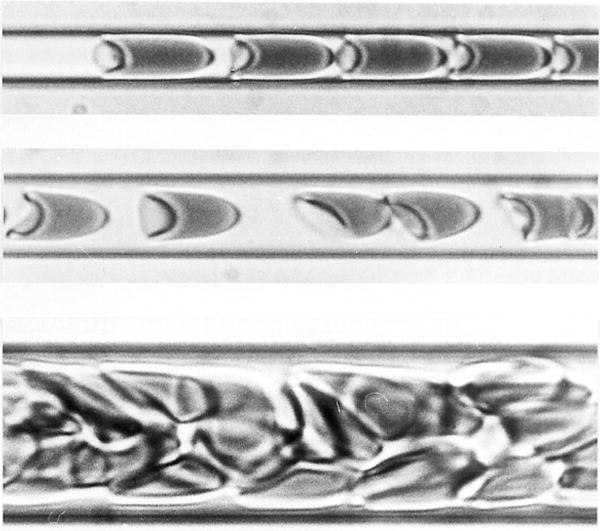
\includegraphics[width=\textwidth, height=5.3cm]{cropped-RBC-in-capillaries.jpg}
    \caption{}
    \label{fig:rbc-in-tubes}
  \end{subfigure}
  \hfill
  \begin{subfigure}[b]{.45\textwidth}
    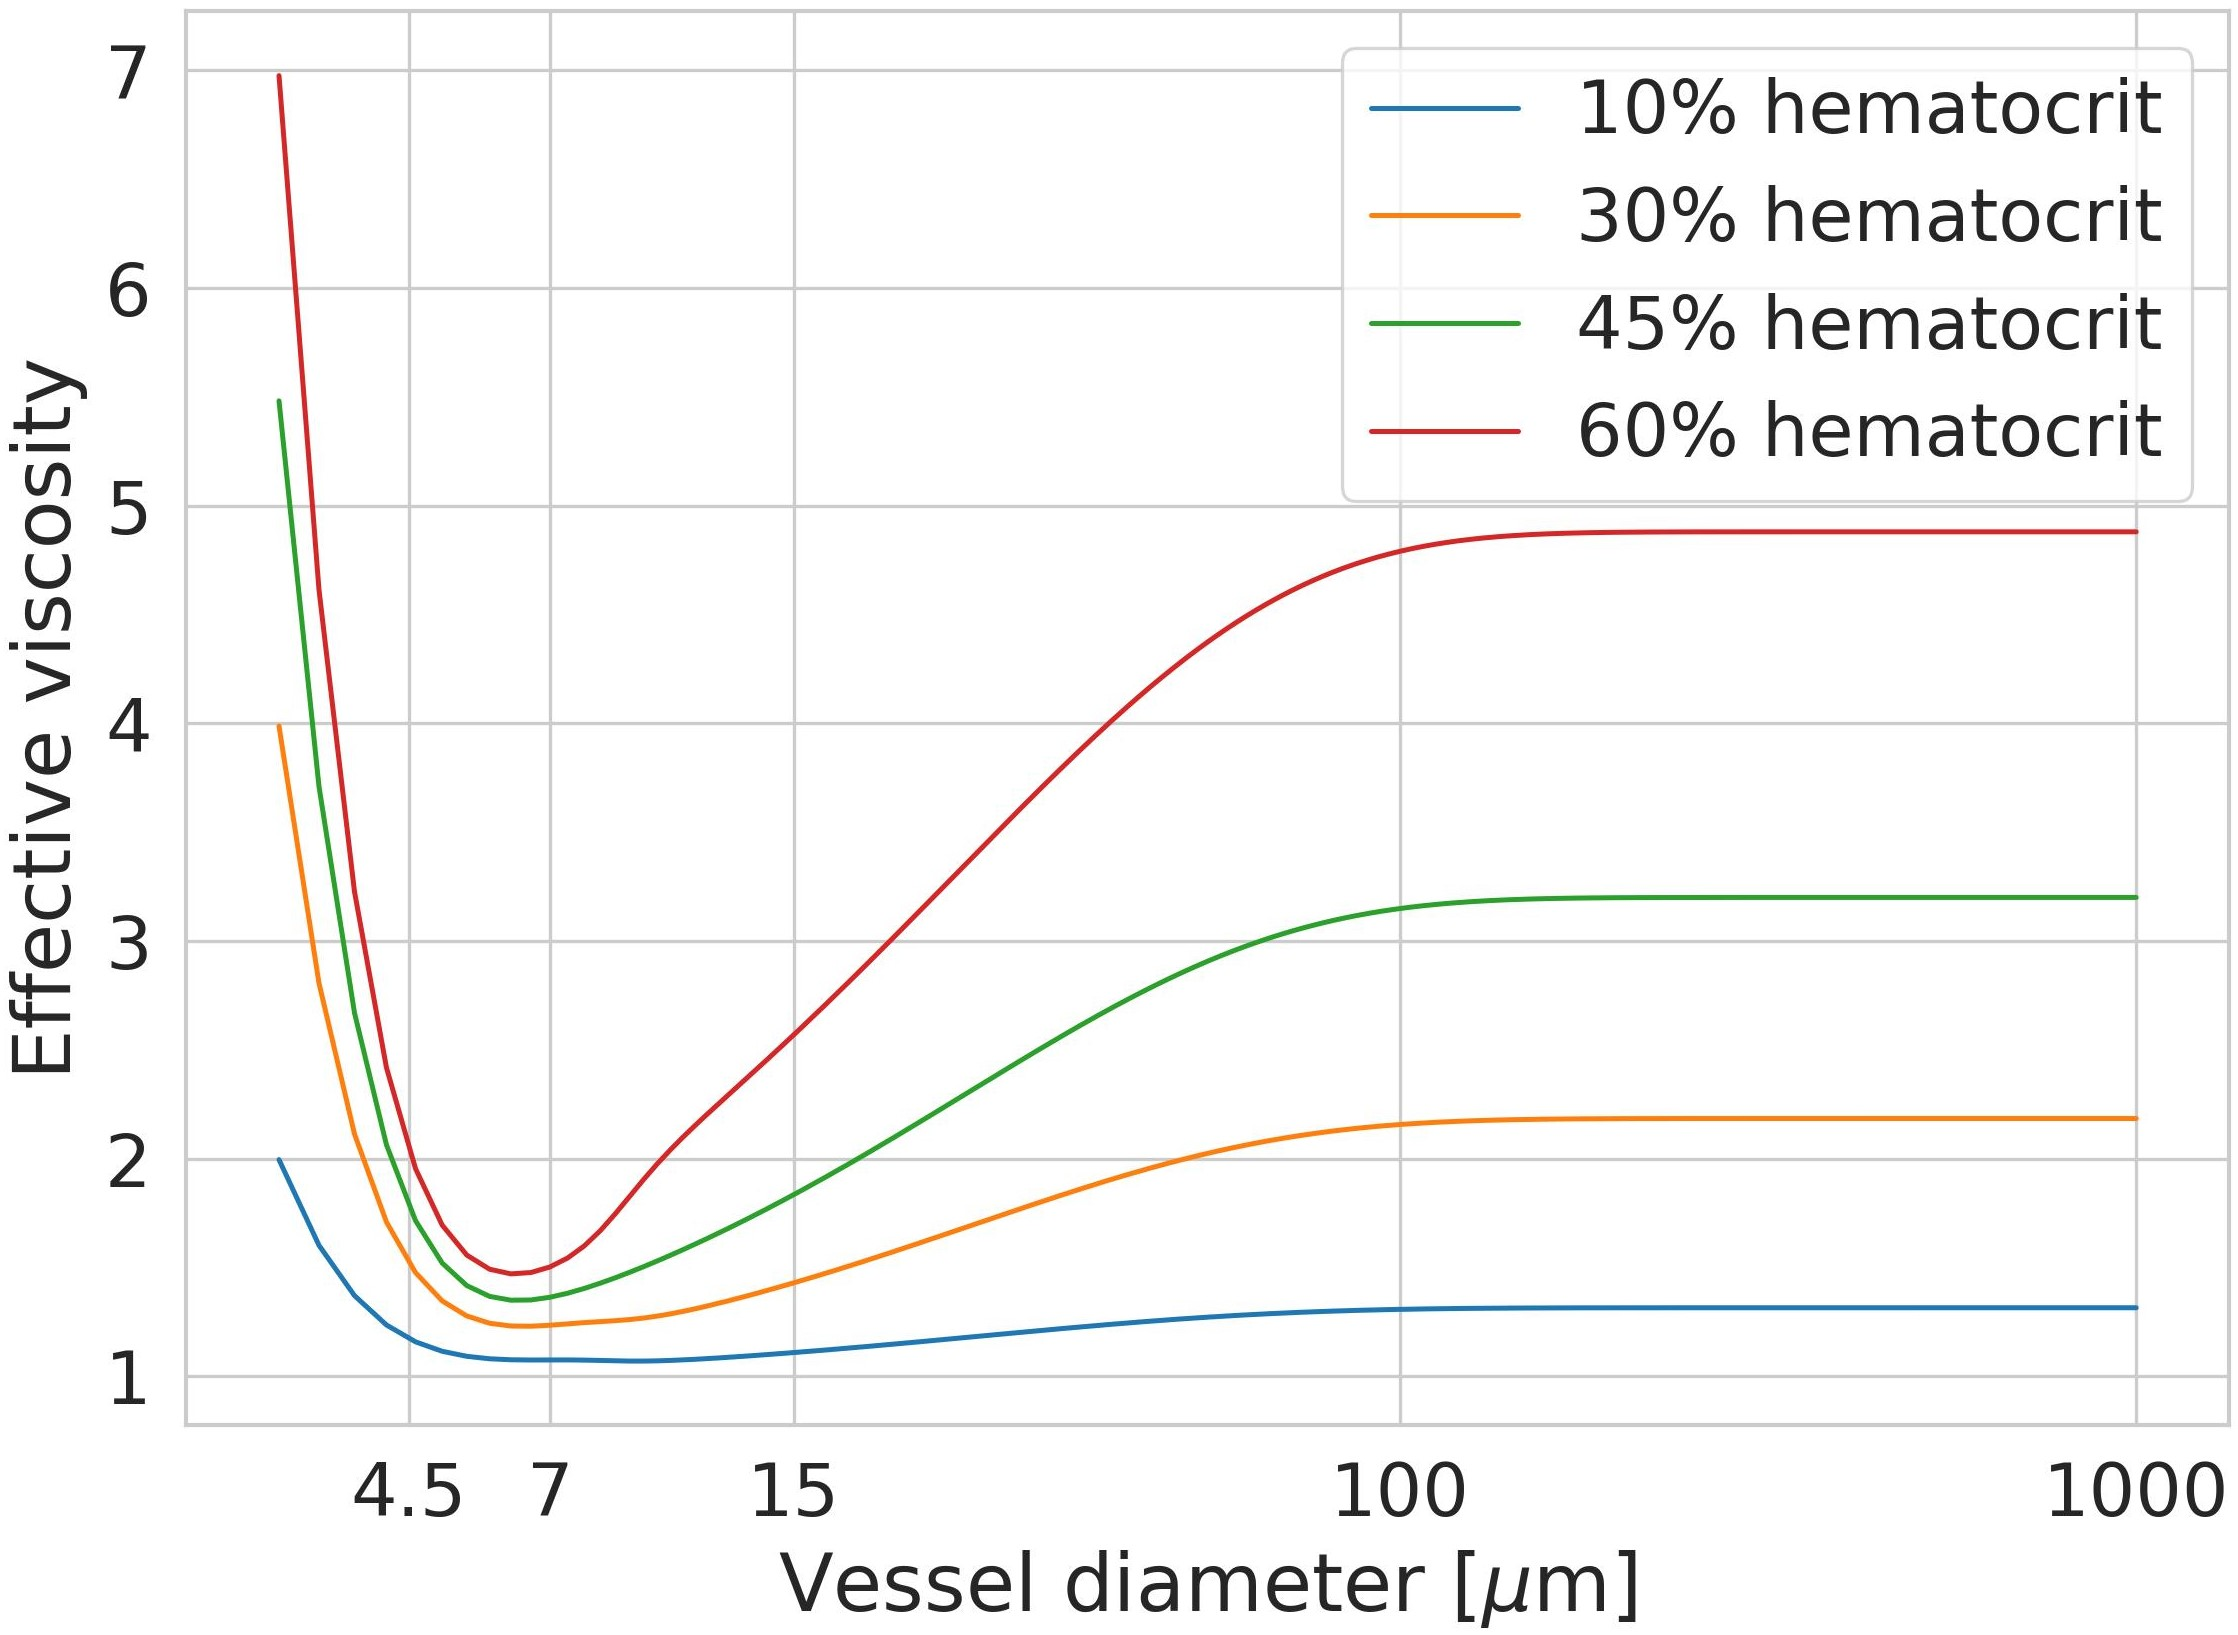
\includegraphics[width=\textwidth]{EffectiveViscosity-Secomb.jpeg}
    \caption{}
  \end{subfigure}
  \caption{Example of the effect of capillary calibre on the flow of blood. (a): Red blood cells in suspension in blood flowing within tubes of different diameter: \SI{4.5}{\micro\meter} (top), \SI{7}{\micro\meter} (middle) and \SI{15}{\micro\meter} (bottom). One can observe the flow of cells converging into a single file, surrounded by a layer of plasma as the diameter moves from \SI{15}{\micro\meter} to \SI{7}{\micro\meter}. The cell's shape adapt to fit into the tube as the diameter reaches the cell's size (top row). Image taken from~\cite{Secomb_2013} \textbf{(not the right reference)}. (b): Example of an empirical law for the effective viscosity of blood accounting for the F\r{a}hr\ae us-Lindqvist effect and increased vascular resistance in smaller capillaries from the work of Secomb and Pries~\cite{Secomb_2013}.}
  \label{fig:effectiveViscosity}
\end{figure}

\textbf{==========>}
How those models can be used to estimate parameters to complement in vitro/in vivo measurements.
\begin{itemize}
\item lists the parameters of the system
\item lists the parameters that can be measured somehow (and how)
\item explain we can fit the model to measurements
\item we can deduct other parameters of interest: pressure, shear rate and stress
\item determining baseline parameters (in health) provides a framework on which to add dynamics of a given disease
\item maybe move this paragraph before talking of the equations
\end{itemize}

Blood flow across a section of the vasculature is driven by a pressure drop between both ends of the section.
A section can range from a single vessel to a whole vascular bed.
This relationship between the blood flow $Q$ and the pressure drop $\Delta p$ is linear, namely $\Delta p\propto Q$.
However, the proportionality constant in this relationship is given by a vessel's or a group of vessels' resistance to the flow.
This vascular resistance $\mathcal{R}$ is nonlinearly dependent on blood and vessel characteristics.
In particular, the fourth power of the radius, $r^4$, appears in this relationship, meaning that even small variations in vessel radius have a strong influence on the flow of blood.
Another important parameter affecting blood flow is the blood's viscosity, noted $\mu$.
Among those parameters, and in the case of the retina, radius and length of vessels can be measured \textit{in vivo} with angiographic devices such as OCTA.
However, this task is more complicated in the choroid.
Blood pressure at the entrance of the retina and the choroid can be estimated from systemic blood pressure and intraocular pressure \textbf{References here. Also, is this estimate taken from haemodynamics models results?9}. 
On the other hand, blood viscosity cannot be measured \textit{in vivo}.



\textit{This framework to model blood flow allows researchers to estimate healthy retinal haemodynamics parameters across the vascular network.
By varying the parameters of each models, it is then possible to simulate diseased conditions for the retinal perfusion.
Investigating the effect of a disease on the perfusion of the retina helps linking clinical observations with cellular scale degenerations.}
\textbf{\\<===========}

\subsubsection{Healthy retina}

To the best of our knowledge, the first haemodynamic model of the retinal microcirculation is a work done by Takahashi et al.~\cite{Takahashi_2009}.
Their aim was to estimate the distribution with respect to vessel caliber of haemodynamic parameters in the human retinal microvasculature.
In this work, the arterial tree is approximated by a dichotomous branching tree, with each generation of vessels branching into two vessels, starting from the central retinal artery.
Radius of the daughter vessels is determined by Murray's theoretical law~\cite{Murray_1926}:
\begin{equation}
  \label{eq:MurrayLaw}
  r_p^\gamma = r_{d,1}^\gamma + r_{d,2}^\gamma
\end{equation}
with $r_p$ the parent vessel radius and $r_{d,i},~i=1,2,$ the radius of the daughter vessels.
The exponent $\gamma$ was determined theoretically by Murray to be equal to $3$, however Takahashi et al. used $\gamma=2.85$ as suggested by more recent work.
After branching dichotomously fourteen times, each of the terminal arterioles sprout four capillaries of fixed homogeneous caliber. 
The venous tree is created symmetrically, starting from the central retinal vein to reach the capillary level where both trees are linked together, for a total of almost $10,000$ vessels in the network.\\
Since the vessels are assumed cylindrical and long with a constant cross section for each generation, the Poiseuille law can be used to describe the pressure drop along each vessel.
The viscosity model used in this paper does not account for increased vascular resistance in capillaries~\cite{Haynes_1960}. \\
% This work provides an initial estimate of the distribution of haemodynamic parameters in the arterio-venous network in the retina. \\
This work provides an simple estimate of how haemodynamic parameters vary with position across arterioles, capillaries and venules.  
It was validated geometrically by comparing the aspect ratio at branches of the arteriolar tree to data from fluorescein photographs of the retina. 
However, it is likely that its efficiency is higher than actual networks since it is generated based on optimality principles and does not include the influence of varying external and internal pressures on the blood flow.
Indeed, several experimental and \textit{in silico} studies have shown that variations in intraocular pressure (IOP) and ocular structure cause strong variations of the haemodynamics of the central retinal artery and, consequently, the downstream vasculature~\cite{Guidoboni_2014, Harris_1996}.

Guidoboni et al. proposed a model that accounts for such variations through a coupling of haemodynamic and mechanistic models of the insertion of the central retinal artery into the retina~\cite{Guidoboni_2014}.
The central retinal artery travels in the optic nerve canal to enter the retina and is subject to two opposing forces: the cerebrospinal fluid pressure and the intraocular pressure.
Harmful effects on blood flow in the artery caused by the pressure difference are prevented by the lamina cribrosa that surrounds the vessel when crossing the sclera.
By modelling the pressure induced on the vessel, they were able to estimate displacement of the vessel wall along the optic nerve length and the impact on blood flow in the artery in both baseline and elevated IOP conditions.\\
The lamina cribrosa is modelled as a circular plate.
The plate is subject on its boundaries to stress from the IOP, cerebrospinal fluid and the sclera and is assumed to behave as a nonlinear, homogeneous, isotropic and elastic material.
The resulting stress tensor acts linearly on the outer part of the vessel wall, with the vessel assumed to be a hollow cylinder passing through the center of the lamina cribrosa.
On the inner surface, the displacement of the wall is provoked by the blood flow within the artery.
Finally, blood flow within the artery is modelled as a Newtonian, incompressible viscous fluid with negligible radial velocity within a cylinder of varying cross section.\\
Across the range of normal intraocular pressures, between $15$ and $20$ mmHg, the model predicted a decrease of almost $5\%$ in blood flow rate.
Variations in the dimension of the sclera and lamina cribrosa can also induce strong reductions of blood flow, particularly in case of elevated IOP. \\

In addition to structural mechanical forces, the vascular blood flow is influenced by variation of vascular resistance due to change in tone of the smooth muscle cells lining the vessel walls.
This reaction may be triggered by variations in systemic blood pressure, metabolic demand, arterial blood gases or intraocular pressure.
Due to the changes in structure and function of the blood vessels and the tissue surrounding it, the mechanisms of blood flow regulation may become altered, leading to increased stress and ischemia in the tissue.
These conditions are ideal for the onset of neovascularisation and edema.
For a detailed review of blood flow in the retina and its regulation in health and disease, see~\cite{Pournaras_2008} and references therein.
While experiments show the importance of blood flow regulation in the retina, the effects of individual regulatory pathways are difficult to investigate \textit{in vivo}. 
Therefore, including auto-regulation and the signaling pathways that lead to the contraction or dilation of vessels in haemodynamic models is essential to understand the mechanisms of auto-regulation and their implication in diseases.
Such models provide an insight into the mechanisms leading to clinical observations and should be accounted for in updated theories of the pathogenesis of certain diseases~\cite{Petersen_2019, Wang_2014}.

Following their previous work, Guidoboni et al.~\cite{Guidoboni_2014b} built up on this model of the central retinal artery by including arterioles, capillaries and venules up to the central retinal vein.
This 0-dimensional model uses the network proposed by Takahashi et al.~\cite{Takahashi_2009}, aggregated into compartments for arterioles, capillary, venules and central retinal vein.
Following an analogy with electrical circuits, different resistance and capacitance properties apply for each compartment.
These characteristics of an electrical circuit's components represent the vascular resistance opposing the flow and the capacity to store blood volumes and deform.
Applying Ohm's law to the network results in a system of ordinary differential equations involving the time derivatives of transmural pressure (the difference in pressure between either side of a vessel wall) in each compartment.
Time dependence emerges from inlet at the central retinal artery which follows a typical cardiac cycle.\\
Both a passive and active mechanism of blood flow regulation are introduced in this model through variable resistances.


First, the vascular resistance of a given compartment varies in a passive way through deformation caused by the transmural pressure $\Delta P$ according to:
\begin{equation*}
  \label{eq:PassiveVariableResistance}
  \mathcal{R} = \frac{8\pi\mu L}{A^2_{ref}}\left(1+\frac{\Delta P}{k_pk_L}\right)^{-4},
\end{equation*}
where $A_{ref}$ is the reference cross section area of the vessel when $\Delta P = 0$, $L$ is the length of the vessel and $k_p,~k_L$ are coefficient defining the deformability of the vessel.
Additionally, to account for the possibility of vein collapsing, $\Delta P$ is allowed to take negative values for veins and venules, in which case the resistance is given by:
\begin{equation*}
  \label{eq:PassiveVariableResistanceCollapse}
  \mathcal{R} = \frac{8\pi\mu L}{A^2_{ref}}\left(1-\frac{\Delta P}{k_p}\right)^{4/3},\qquad \text{for } \Delta P<0.
\end{equation*}
By contrast, blood flow auto-regulation through smooth muscle cells is accounted for by a phenomenological model of the vascular resistance in arterioles.
Absence of auto-regulation is assumed to correspond to a constant resistance $R_{ref}$.
The flow computed for a given ocular perfusion pressure (OPP) at the central retinal artery gives a baseline value $Q_{baseline}(OPP)$ from which the active resistance is computed according to:
\begin{equation*}
  \label{eq:ActiveResistancePhenomenological}
  \mathcal{R}_{arteriole} = \mathcal{R}_{ref}\frac{c_L + c_u\exp\Bigl(K\bigl(Q_{baseline}(OPP)- Q\bigr)-\hat c\Bigr)}{1 + \exp\Bigl(K\bigl(Q_{baseline}(OPP)- Q\bigr)-\hat c\Bigr)}.
\end{equation*}
With OPP varying throughout a cardiac cycle, the mean model-predicted blood flow across the vascular network matches experimental values for a range of healthy mean arterial pressures.
Using this model, one can predict based on systemic blood flow measurements (e.g., mean arterial pressure) what range of intraocular pressure a simulated retinal vasculature can handle while limiting the disruption of vascular functions in the retina.
Simulations can recreate patients with working or defective auto-regulation system as well as hypertensive (blood pressure anormaly high) or hypotensive (blood pressure anormaly low) patients, both aspects being common in age and disease.
In particular, hypertension is a common risk factor to a number of retinal diseases, e.g., as AMD and glaucoma, though the links with the onset of retinopathies are not well understood~\cite{Klein_2004, Leeman_2019}.

While the previous model by Guidoboni et al.~\cite{Guidoboni_2014b} models varying vascular resistance with a phenomenological approach, Arciero et al.~\cite{Arciero_2013} chose a mechanistic modelling approach of the various signals acting on smooth muscles tone.
The mechanisms triggering auto-regulation included in this work are: pressure, shear stress on the vessel wall, metabolic response, local tissue concentration of carbon dioxide and neural stimuli.
The idea of the model was to investigate the implications of each auto-regulation pathways, individually and collectively, in glaucoma.
Glaucoma is characterized by degenerations of the optic nerve and the retinal ganglion cell layer and is associated with impairments of the vascular system, both in the systemic and retinal circulation, and with elevated intraocular pressure~\cite{Bonomi_2000, Hulsman_2007}.

In the studies presented before, the vasculature is represented in a simplified way, either as compartments with varying resistance and capacitance or generated following optimality principles.
However, retinal angiograms have shed light on a number of vascular biomarkers retinal and neurogenerative diseases~\cite{Chalam_2016,Tsokolas_2020}.
Despite their clinical relevance, the exact relationship between those biomarkers and the development of retinal pathologies is still unclear.
Therefore, some groups tried to simulate haemodynamics in vascular trees segmented from retinal angiograms~\cite{Aletti_2016, Liu_2009, Malek_2015, Rebhan_2019}.
However, they are for most limited to small segments of the arterial network, hence ignoring the effect of downstream capillaries and venules in the distribution of haemodynamic parameters or including the remaining vessels as compartments, as previously described.

Despite the limitations and difficulties, these works provide a framework to investigate oxygen delivery and stress associated with ageing in vasculature and tissue that may affect visual function~\cite{Rickett_2010,Sim_2013,Wessel_2012}.
Notably, Rebhan et al. proposed a framework to investigate tissue stress induced by blood flow, an aspect of research still unexplored~\cite{Rebhan_2019}.

\break

\subsubsection{Ageing and diseased retina}


The effects of age and disease on the vasculature can be readily observed and quantified on retinal angiograms and structural images.
In particular, vessel density and larger capillary-free areas in the inner retina have been related to severity of the disease in glaucoma, diabetic retinopathy and neovascular age-related macular degeneration~\cite{Al_Sheikh_2016, Rao_2020, Yuan_2020}.
In those diseases, retinal cell layers appear affected by changes in the vasculature.
One reason is the reduced perfusion that creates ischemia in the tissue.
Retinal non-perfusion areas can be visualized on angiograms, however, the exact availability of oxygen in the tissue can hardly be measured \textit{in vivo}.
Additionally, with age, blood vessels tend to work at full capacity in term of blood flow.
This leads to first, the loss of auto-regulation capabilities and second, additional stress on the blood vessels and the tissue within which they are embedded.\\
Mechanical stress and its relation to diseases can be investigated \textit{in silico}.
Rehban et al. proposed such a model based on segmented vasculature~\cite{Rebhan_2019}.
Their finite element approach uses very fine grid elements to embed vessels directly into a retina with different mechanical properties for cell layer.
The combination of haemodynamics in a segmented vascular network and the embedding in tissue provide direct insight in the stress acting on the tissue and vessel walls for different subjects.
The vascular network of an healthy subject, a subject with DR and a subject with glaucoma were used for comparison.
The inlet flow for each case was scaled accordingly to the subject specifities.
The experiments showed important differences in wall shear stress between each groups, with diseased cases being subject to higher stress.
This was true for all vessel diameters.\\
Guidoboni et al. used their theoretical vascular network to investigate the range of intraocular pressure that patients suffering from low or high systemic blood pressure or loss of auto-regulation function can withstand with limited variation of retinal blood flow~\cite{Guidoboni_2014b}.
Their model suggest that the extend of the effect of IOP on haemodynamics is influenced by both, an individual's arterial blood pressure and capacity to auto-regulate blood flow.
They concluded that the complex relationship highlighted by the model may explain the difficulty to obtain consistent results from \textit{in vivo} experiments.


%%%% Part on the choroid
While the inner retinal vasculature feeds the inner third of the retina, the remaining two thirds are perfused by the choroidal circulation.
In contact with the retina is the choriocapillaris (CC) layer of the choroid.
The CC provides oxygen across the Bruch's membrane to the photoreceptors and other neuronal cells of the outer retina through diffusion only.
Therefore, a high vascularization is necessary to provide enough oxygen across the distance.
Defects in choroidal blood flow are associated with major retinopathies such as nAMD and DR~\cite{Pemp_2008}.
In particular, reduction of choroidal perfusion is believed to be a major factor in the development of neovascularization.
Despite its importance, little is known about the choroid and its haemodynamic given its location behind the retina that makes it less accessible for measurements. 
Similarly, little work has been done on modelling the haemodynamic of the choroid.
Zouache and colleagues attempted to close this gap by modelling the choriocapillaris and its peculiar architecture~\cite{Zouache_2015}.
By simulating the lobular structure of the CC, they investigated the effects of the geometry of an individual lobule on the blood flow.
Their work suggested that the distribution of flow separators in the CC and the location of inlet and outlets in individual lobules may explain the localization of edema or neovasculature in diseased eyes.
Other than the work of Zouache et al., Flower and colleagues theoretically determined the amount of photocoagulation therapy necessary to treat choroidal neovascularization in~\cite{Flower_2001}.
This therapeutic approach has however now been mostly replaced by intravitreal injections of antiVEGF agents.


\subsection{Anti-VEGF therapy}
Coming soon.
\subsection{Laser treatment}

% \begin{spacing}{0.0}
\bibliographystyle{abbrvnat} % {ksfh_nat}
{\normalsize \bibliography{Haemodynamics_nAMD_DR}}
% \end{spacing}

\end{document}
